% From assignment:
% Prioritize measurements and analysis/interpretation!

% Demonstrate use of tools (profiling, ...) , and simple performance
% model.

\section{Measurements}

We used Valgrind performance tools to determine where the C++ code
spends execution time, \texttt{Rprof} to analyse the R code and simple
printed timings to analyse the performance of the whole simulation. 

\subsection{Motivational R-side measurement}

\begin{figure}[!htbp] \centering
  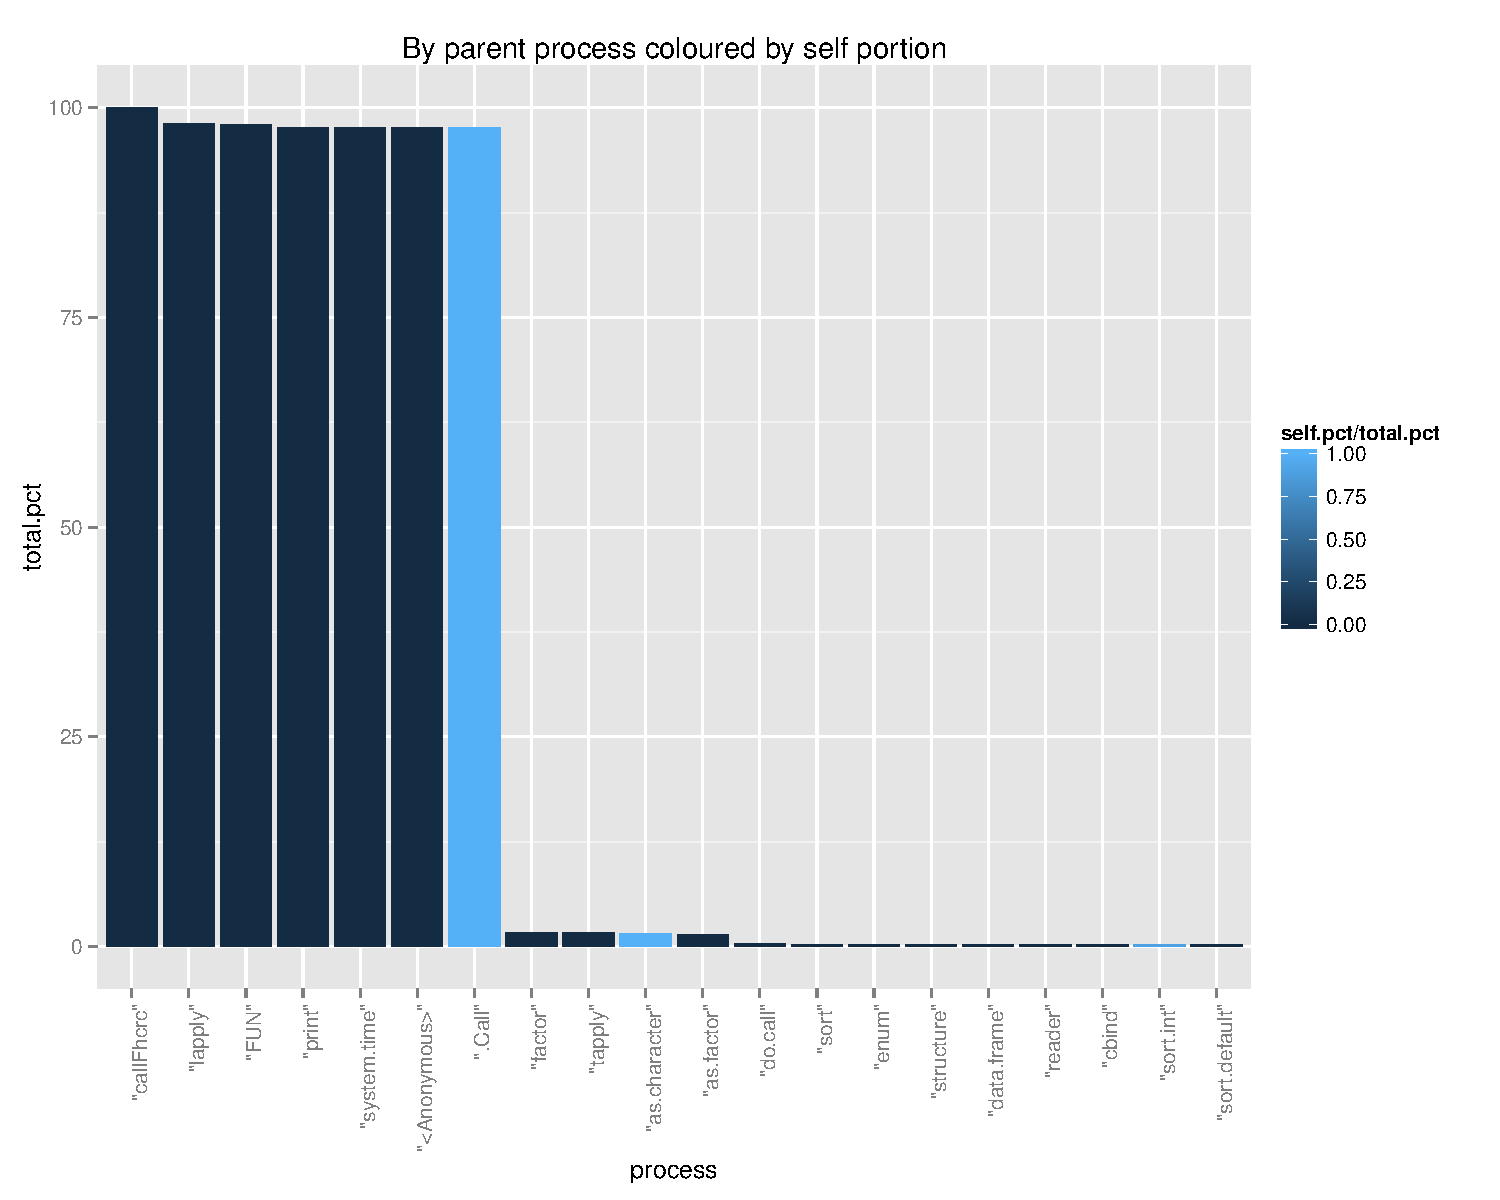
\includegraphics[width=0.7\textwidth]{images/parentColByPortion.pdf}
  \caption{Performance testing on the R side, where the "\texttt{.Call}" is the
C++-code which can be run in parallel.}
  \label{fig:rMot}
\end{figure}

To motivate the need, and to decide what part to parallelise, we made
an initial performance measurement form the R-side perspective of the
program. Figure \ref{fig:rMot} shows the processes from the R-side
where ``\texttt{.Call}'' is the part which is implemented in C++ and
which can be rewritten as a parallel program given the techniques
presented in the course. The height of the bars indicates the total
time spent in the call to the function, and the brighter the colour
the more time is spent in the actual function. From Figure
\ref{fig:rMot} we can conclude that ``\texttt{.Call}'' itself
constitutes over 95\% of the program execution time.

\subsection{Motivational C++-side measurement}
\begin{figure}[!htbp] \centering
  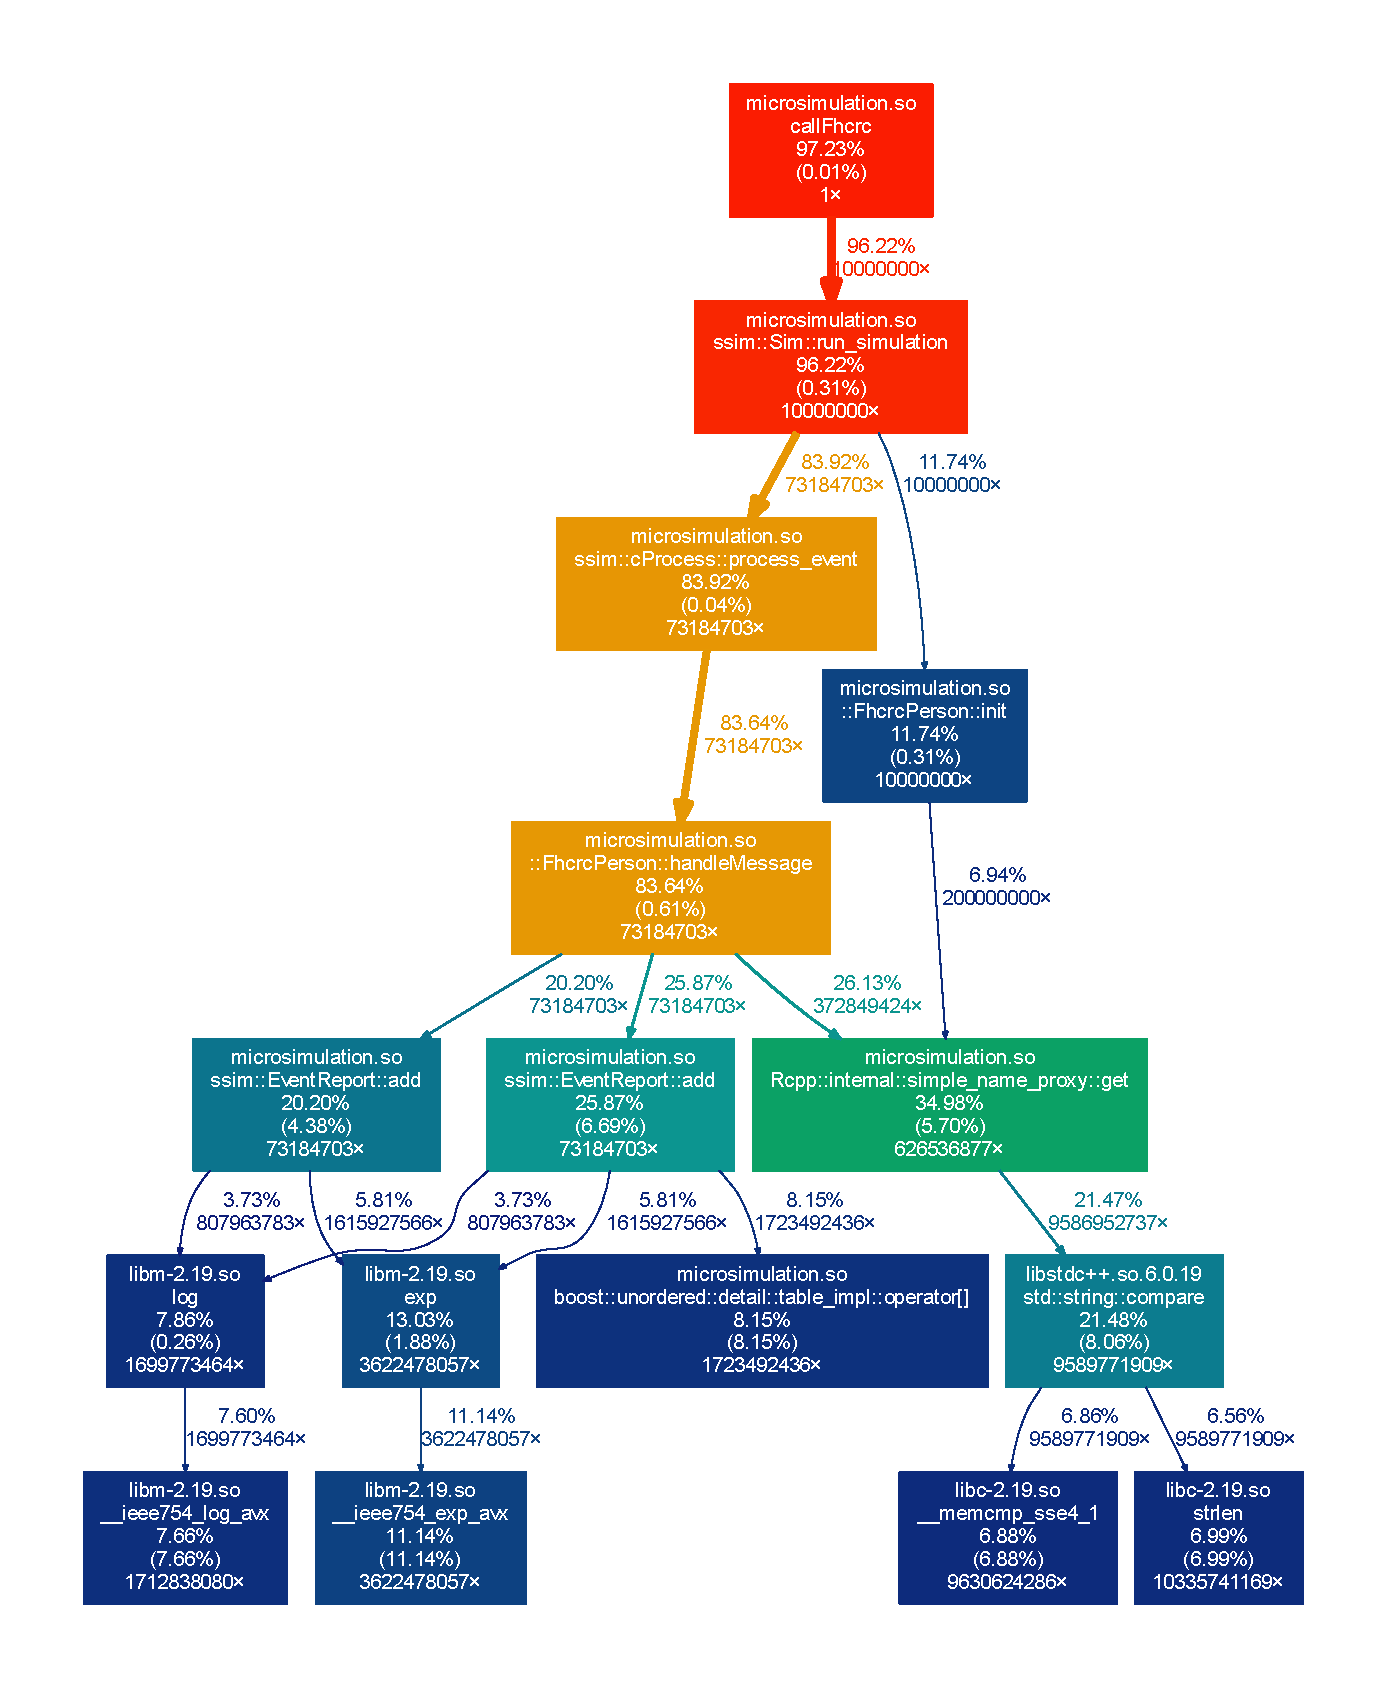
\includegraphics[height=0.70\textheight]{images/simpleMotivatingValgrind.pdf}
  \caption{Using Valgrind to profile the main C++ function. This
    function is possible to parallelise.}
  \label{fig:cppMot}
\end{figure}
We used Valgrind to profile the C++ function, ``\texttt{callFhcrc}'',
that is called in ``\texttt{.Call}'' from the R-side. Figure
\ref{fig:cppMot} shows the most significant parts of the output from
this profiling. This function is called once for each simulated
individual and is possible to run in parallel. Noteworthy is that
almost half of the execution time is spent in the
\texttt{EventReport::add} method function. This function is
collecting, i.e., reducing, the results from the individuals in the
simulation to categories and stores them in a dynamically allocated
associative array. For a more detailed version see Figure
\ref{fig:mediumValgrind} in Appendix \ref{sec:valgrind} and for the
full profiling see
\url{https://github.com/mclements/microsimulation/blob/sim_instances/analysis/fullProfilingNotForPaper.pdf}.


%%% Local Variables: 
%%% mode: latex 
%%% TeX-master: "report" 
%%% End:
